\documentclass{article} % For LaTeX2e
\usepackage{iclr2026_conference,times}

% Optional math commands from https://github.com/goodfeli/dlbook_notation.
\input{math_commands.tex}

\usepackage{amsmath}
\usepackage{amssymb}
\usepackage{array}
\usepackage{booktabs}
\usepackage{float}
\usepackage{graphicx}
\usepackage{hyperref}
\usepackage{url}

\title{Optimizer-Conditioned Geometry for Feature-Based Uncertainty}

% Keep the submission anonymous while \iclrfinalcopy is commented.
\author{Anonymous Authors}

% Uncomment only for the accepted camera-ready version.
% \iclrfinalcopy

\begin{document}

\maketitle

\begin{abstract}
Modern classifiers are often selected by in-distribution accuracy, yet
downstream reliability can depend on geometric properties of the learned
representation that accuracy does not reveal. This is especially important for
feature-based uncertainty and out-of-distribution (OOD) detectors, which read
distances, norms, covariances, and local neighborhoods in the penultimate
feature space. We study whether optimizer choice preserves the geometry required
by these detector families. Rather than proposing a new detector, we use SGD,
Adam, and AdamW as controlled interventions on representation geometry and
evaluate how their optimizer-induced feature profiles are read by logit-based
and feature-based OOD scores. In accuracy-controlled selected configurations on
CIFAR-10 with WideResNet-28-10, we find that models with comparable ID
performance can exhibit distinct penultimate geometry fingerprints, including
differences in neural-collapse metrics, feature norms, within-class dispersion,
and class separation. These differences are not uniformly reflected in detector
behavior: logit-based scores can remain competitive while raw Mahalanobis and
kNN scores degrade substantially in AdamW-selected regimes. Post-hoc L2
normalization recovers much of this raw feature-detector gap, indicating that
radial or norm-coupled geometry is a major failure channel, while
covariance-side controls show more limited and detector-dependent effects. Our
results therefore do not support an optimizer-good/bad ranking. They support a
geometry--detector compatibility view: optimization improvements may preserve,
distort, or mask the representation geometry required by a downstream
uncertainty estimator. This controlled study suggests that optimizer choice
should be evaluated jointly with penultimate geometry and detector-family
readout, not by ID accuracy alone.

\end{abstract}

\section{Introduction}
\label{sec:introduction}
Deep neural networks are commonly selected by in-distribution (ID) accuracy.
This criterion is natural for closed-set recognition, but it is not sufficient
for reliable deployment. In open environments, a model must also assign useful
uncertainty to ambiguous inputs, low-confidence cases, and samples that do not
come from the training distribution. Out-of-distribution (OOD) detection addresses
this problem by assigning a score that separates ID-like inputs from unreliable
or shifted inputs. However, different OOD scores do not read the same part of a
trained model. Logit-based scores such as maximum softmax probability (MSP),
MaxLogit, and Energy read output confidence, logit scale, and margin structure
\citep{hendrycks2017baseline,liu2020energy}. Feature-based scores instead read
the penultimate representation through distance, density, neighborhood, angular,
or subspace structure
\citep{lee2018simple,sun2022knn,mukhoti2021ddu,nguyen2023ctm,benammar2023neco}.
Thus, OOD reliability is not determined only by the score formula; it also
depends on the geometry of the representation on which the score is applied.

This observation raises a question that is largely hidden when optimizers are
treated only as tools for improving accuracy. Optimizer choice can change the
implicit bias of training and therefore the geometry of the learned
representation. Recent work on Neural Collapse shows that optimizers and
weight-decay coupling can substantially affect last-layer and penultimate
geometry, with SGD, Adam, and AdamW exhibiting different collapse behavior
\citep{papyan2020prevalence,zhao2026optimizer}. In particular, the distinction
between coupled and decoupled weight decay is not merely an implementation
detail: it can change the dynamics by which class means, classifier weights, and
feature clouds organize during training \citep{loshchilov2019decoupled}. If
feature-based OOD detectors depend on this geometry, then optimizer choice may
affect OOD detectability even when ID accuracy is comparable.

We study this optimizer--geometry--detector interaction. Our central hypothesis
is that optimizer choice induces a penultimate geometry fingerprint, and that OOD
detector behavior depends on whether this fingerprint is compatible with the
geometry channel read by the detector. Under this view, there need not be a
universally best optimizer or a universally best detector. The relevant object is
the compatibility between the optimizer-induced representation and the
detector-family readout. Figure~\ref{fig:optimizer-geometry-pipeline}
summarizes this optimizer-conditioned geometry compatibility framing.

\begin{figure}[t]
\centering
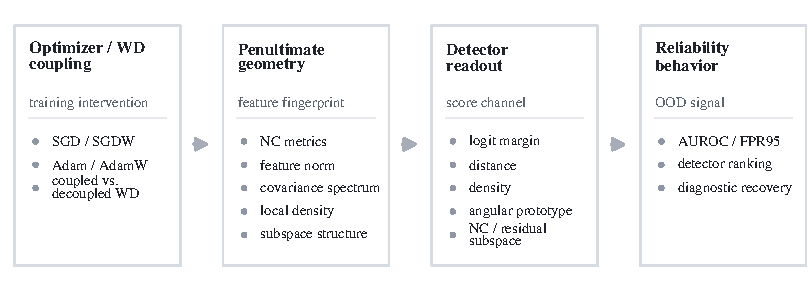
\includegraphics[width=0.98\linewidth]{figures/fig1_optimizer_geometry_pipeline.pdf}
\caption{Optimizer-conditioned geometry compatibility. Optimizer and
weight-decay-coupling choices shape penultimate feature geometry, and detector
families read different channels of that geometry. Diagnostic controls localize
whether detector changes are carried by radial, covariance, neighborhood,
angular, or subspace structure.}
\label{fig:optimizer-geometry-pipeline}
\end{figure}

We evaluate this view using SGD, SGDW, Adam, and AdamW as controlled optimizer
families. This choice separates two axes that are often conflated: adaptivity
and weight-decay coupling. SGD and SGDW compare coupled and decoupled decay in a
non-adaptive optimizer, while Adam and AdamW compare the same distinction under
coordinate-wise adaptive updates. To test whether the resulting geometry effects
are architecture-specific or more general, our study is organized around
convolutional backbones with different inductive biases, including non-residual,
residual, and modern CNN architectures. Transformer-based architectures are
treated as robustness settings, where pretraining, normalization layers, and
token-based representations may change how optimizer effects appear.

A key part of our study is to separate detector performance from diagnostic
interpretation. We do not introduce normalization, covariance stabilization, or
projection as new OOD detectors. Instead, we use them as controlled interventions
that remove or stabilize specific geometry channels. If a detector gap disappears
after such an intervention, the corresponding channel is implicated; if the gap
remains, the mismatch likely involves broader representation structure. The
formal readout map and the diagnostic recipe are developed in
Section~\ref{sec:method}, with full score and metric definitions provided in the
appendix.

This framing differs from a standard OOD benchmark. Rather than asking which
detector wins on average, we ask why detector rankings change when the
representation changes. Representation-centric analyses have shown that OOD
detector competitiveness depends on architecture, training paradigm, source
dataset, and shift severity \citep{olivares2025systematic}. We focus on one
specific and actionable source of such variation: optimizer choice. By measuring
the geometry exposed by a trained classifier and comparing how detector families
respond, we connect optimizer-induced representation changes to downstream
feature-based uncertainty behavior.

Our contributions are as follows.
\begin{itemize}
    \item We formulate optimizer-conditioned geometry compatibility as a lens for
    feature-based OOD detection: optimizer choice shapes the penultimate geometry
    that downstream detector families read.

    \item We study SGD, SGDW, Adam, and AdamW as controlled interventions that
    separate adaptivity from weight-decay coupling, and evaluate how these choices
    change detector-relevant representation geometry.

    \item We connect optimizer-induced geometry fingerprints to detector-family
    behavior, showing why comparable ID accuracy need not imply comparable
    feature-based uncertainty.

    \item We use diagnostic controls to localize whether detector changes are
    carried by radial, covariance, neighborhood, angular, or subspace channels,
    supporting a compatibility view rather than an optimizer leaderboard.
\end{itemize}


\section{Related Work}
\label{sec:related-work}
\subsection{Optimizer-Induced Neural Collapse and Feature Geometry}
\label{subsec:optimizer-geometry}

Neural Collapse provides a geometric description of the terminal phase of
supervised training, in which penultimate features, class means, and classifier
weights approach a highly structured configuration
\citep{papyan2020prevalence}. This perspective is useful for reliability because
it separates accuracy from representation geometry: two classifiers can achieve
similar ID performance while differing in within-class compactness, class-mean
separation, classifier--feature alignment, feature-norm structure, and covariance
shape. Feature-based OOD detectors operate precisely on these geometric
quantities, so changes in Neural Collapse or related feature geometry can affect
detector behavior even when classification accuracy is comparable.

Recent work shows that this geometry is not optimizer invariant.
\citet{zhao2026optimizer} demonstrate that optimizer choice and weight-decay
coupling affect the emergence of Neural Collapse, with SGD, Adam, and AdamW
exhibiting different collapse behavior. This is closely related to the distinction
between coupled and decoupled weight decay \citep{loshchilov2019decoupled}. In
SGD-like optimizers, coupled and decoupled decay can be relatively similar in
their practical effect, whereas in adaptive optimizers the distinction can change
the implicit bias of training. Our work builds on this optimizer-to-geometry
view, but studies the next step: how geometry differences induced by SGD, SGDW,
Adam, and AdamW are inherited by downstream OOD detector families.

\subsection{Feature-Based OOD Detectors as Geometry Readouts}
\label{subsec:feature-based-ood-readouts}

OOD detection methods assign scores intended to separate ID-like inputs from
unreliable or out-of-distribution inputs. Logit-based scores such as MSP,
MaxLogit, and Energy read output confidence, logit scale, and margin structure
\citep{hendrycks2017baseline,liu2020energy}. They are useful and often strong
baselines, but they do not directly model the geometry of the penultimate feature
space.

Feature-based detectors instead read different geometric channels of the learned
representation. Mahalanobis scoring fits class means and covariance estimates and
uses a precision-weighted distance to the closest class center
\citep{lee2018simple}. kNN scoring compares a query feature to a bank of ID
training features and is therefore sensitive to local neighborhood spacing,
feature normalization, and local density structure \citep{sun2022knn}. DDU-style
Gaussian density scores fit class-conditional feature densities and read both
distance-to-mean and covariance-volume information \citep{mukhoti2021ddu}.
Angular detectors such as CTM use cosine similarity to class-typical feature
directions \citep{nguyen2023ctm}, while Neural-Collapse-based detectors such as
NeCo use prototype, class-mean, and principal-component structure
\citep{benammar2023neco}. These detectors are therefore not interchangeable
scoring rules: each one reads a different projection of the optimizer-induced
feature geometry.

This readout view is central to our paper. If an optimizer changes feature norms,
raw distance detectors can change even when angular structure is preserved. If it
changes covariance anisotropy or conditioning, Gaussian density and
Mahalanobis-style scores can change even when class means remain separated. If it
changes class-mean directions, classifier alignment, or residual subspaces,
angular and collapse-based scores can change even when raw distance-based scores
appear stable. We therefore organize detectors by the geometry channel they read,
rather than by treating all OOD scores as a single benchmark list.

\subsection{Normalization, Covariance, and Subspace Controls}
\label{subsec:normalization-covariance-controls}

Feature-space preprocessing can substantially change the behavior of
feature-based detectors. In particular, L2 normalization removes radial
feature-norm variation and turns Euclidean comparisons into angular comparisons.
This is important because normalized kNN is often a strong practical variant, and
normalization can also improve Mahalanobis-style scoring when raw feature norms
distort covariance estimates. In our framework, however, the purpose of raw and
normalized variants is not only to compare detector performance. The comparison
itself is diagnostic: raw Mahalanobis and raw kNN expose radial or norm-coupled
geometry, while L2-normalized versions test whether the detector gap remains once
that radial channel is removed.

Covariance-side controls play a complementary role. Mahalanobis and
DDU-style Gaussian density scores depend on covariance estimates, and these
estimates can be sensitive to feature dimension, sample size, anisotropy, and
conditioning. Tied covariance, diagonal covariance, and shrinkage covariance
therefore provide different probes of the same feature distribution. If shrinkage
or diagonalization recovers a detector gap, the failure may be tied to covariance
estimation or ill-conditioning. If the gap remains, the mismatch is more likely
to involve broader representation geometry, such as class overlap, radial
variation, or subspace structure.

PCA-based controls provide another way to separate geometry channels. Projecting
features onto a low-dimensional principal subspace can remove nuisance
directions, while residual-space scores can test whether OOD samples occupy
directions not used by the ID class structure. These transformations are not
introduced here as new detector proposals. Instead, we use them as diagnostic
interventions that help localize whether optimizer-induced detector changes are
carried by radial, covariance, angular, or subspace channels.

\subsection{Representation-Centric Detector Selection}
\label{subsec:representation-centric-detector-selection}

Recent representation-centric analyses argue that detector rankings are not fixed
properties of score formulas. They can change with architecture, training
paradigm, source dataset, representation geometry, and OOD severity
\citep{olivares2025systematic}. This perspective is important for our setting
because optimizer choice is a training-side intervention that can reshape the
representation seen by every downstream detector. A detector that is competitive
under one optimizer-induced geometry may become less reliable under another, not
because the detector formula is intrinsically weak, but because the geometry it
expects has been distorted, masked, or replaced by a different feature regime.

Our work follows this representation-centric view but focuses on a different
source of variation. Rather than varying detector design or training paradigm
broadly, we isolate optimizer choice and weight-decay coupling as mechanisms that
shape penultimate geometry. We then ask whether Neural Collapse metrics,
feature-norm statistics, within-class dispersion, class separation, covariance
spectra, effective rank, and local feature-bank structure can explain or predict
which detector family will work. This turns detector selection into a
geometry-aware diagnostic problem: before choosing a feature-based OOD detector,
one should first inspect the geometry that the trained model exposes to that
detector.

\subsection{Positioning of Our Work}
\label{subsec:positioning}

Prior work provides the components of our argument. Neural Collapse studies show
that final-layer and penultimate features can organize into measurable geometric
structures. Optimizer studies show that this geometry can depend on the training
rule and the coupling of weight decay. Feature-based OOD detectors rely on class
means, covariance, neighborhoods, densities, prototypes, or subspaces.
Representation-centric benchmarks show that detector rankings shift when the
learned representation changes.

The missing link is the optimizer--geometry--detector pathway. We study this
pathway directly by treating SGD, SGDW, Adam, and AdamW as geometry interventions
and by evaluating how their induced penultimate representations are read by
logit-based, distance-based, density-based, neighborhood-based, angular, and
Neural-Collapse-based detectors. The contribution is not another OOD scoring rule
and not a generic optimizer leaderboard. It is a geometry--detector compatibility
framework: optimizer choice should be evaluated jointly with the penultimate
geometry it induces and the detector family that will read that geometry.


\section{Optimizer-Conditioned Geometry and Feature-Based Readouts}
\label{sec:method}
This section defines the mechanistic framework used to analyze how optimizer
choice can affect feature-based uncertainty. We do not introduce a new OOD
detector. Instead, we treat optimizer choice as an intervention on penultimate
representation geometry, and we treat each feature-based detector family as a
readout of a particular geometry channel. The resulting question is not which
optimizer is universally better, but which optimizer-induced geometry is
compatible with which downstream readout.

% TODO: Optional method schematic: optimizer -> geometry fingerprint -> detector readout -> score ranking.

Table~\ref{tab:readout-map} summarizes the detector families considered by this
framework. The table is conceptual: it records which geometry channel each
readout can be sensitive to and which diagnostic control helps localize that
channel.

\begin{table}[H]
\caption{Feature-based detector families as geometry readouts. The entries
summarize the framework only; they do not report experimental results.}
\label{tab:readout-map}
\begin{center}
\footnotesize
\setlength{\tabcolsep}{3pt}
\renewcommand{\arraystretch}{1.15}
\begin{tabular}{@{}>{\raggedright\arraybackslash}p{0.17\textwidth}>{\raggedright\arraybackslash}p{0.25\textwidth}>{\raggedright\arraybackslash}p{0.27\textwidth}>{\raggedright\arraybackslash}p{0.20\textwidth}@{}}
\toprule
Detector family & Score form & Geometry channel & Diagnostic control \\
\midrule
Mahalanobis
& \(-\min_c (f-\mu_c)^\top \Sigma_W^{-1}(f-\mu_c)\)
& class centers, within-class covariance, precision spectrum
& post-hoc L2 normalization; covariance shrinkage \\
Gaussian density
& \(\log\sum_c \pi_c \mathcal{N}(f\mid\mu_c,\widehat{\Sigma}_c)\)
& Gaussian density, covariance volume, anisotropy, conditioning
& tied, diagonal, and shrinkage covariance \\
kNN
& \(-d_k(f,\mathcal{B})\)
& local feature-bank spacing, radial scale, angular neighborhoods
& raw kNN vs. L2-kNN \\
CTM angular readout
& \(\max_c \langle \widehat f,a_c\rangle\)
& prototype or classifier directions, angular class separation
& normalized features; prototype vs. classifier direction \\
NECO collapse/residual readout
& \(\max_c\langle\widehat f,\widehat\mu_c\rangle\), \(-\|(I-P_M)f\|_2^2\)
& collapse-like prototype geometry, residual energy outside class-mean subspace
& prototype vs. residual readout; subspace dimension \\
\bottomrule
\end{tabular}
\end{center}
\end{table}


\subsection{Optimizer-conditioned representation geometry}
\label{subsec:optimizer-conditioned-geometry}

Let \(o\) denote an optimizer or training rule. A classifier trained under
optimizer \(o\) is written as
\begin{equation}
    z_o(x)=W_o f_o(x)+b_o,
    \label{eq:classifier-decomposition}
\end{equation}
where \(f_o(x)\in\mathbb{R}^d\) is the penultimate feature,
\(W_o\in\mathbb{R}^{K\times d}\) is the classifier weight matrix, and
\(z_o(x)\in\mathbb{R}^K\) denotes the logits. Let
\(\mathcal{D}_{\mathrm{tr}}\) be the ID training set and
\(\mathcal{D}_c\subset\mathcal{D}_{\mathrm{tr}}\) be the subset of class \(c\).
For each optimizer \(o\), we define the class mean and covariance in the
penultimate feature space as
\begin{equation}
    \mu_{c,o}
    =
    \frac{1}{|\mathcal{D}_c|}
    \sum_{(x_i,y_i)\in\mathcal{D}_c}
    f_o(x_i),
    \label{eq:class-mean}
\end{equation}
\begin{equation}
    \Sigma_{c,o}
    =
    \frac{1}{|\mathcal{D}_c|-1}
    \sum_{(x_i,y_i)\in\mathcal{D}_c}
    \bigl(f_o(x_i)-\mu_{c,o}\bigr)
    \bigl(f_o(x_i)-\mu_{c,o}\bigr)^\top.
    \label{eq:class-covariance}
\end{equation}
When a detector uses a shared covariance estimate, we use the pooled
within-class covariance
\begin{equation}
    \Sigma_{W,o}
    =
    \frac{1}{K}
    \sum_{c=1}^{K}
    \Sigma_{c,o}.
    \label{eq:pooled-within-covariance}
\end{equation}
We also define the ID feature bank
\begin{equation}
    \mathcal{B}_o
    =
    \{f_o(x_i):(x_i,y_i)\in\mathcal{D}_{\mathrm{tr}}\},
    \label{eq:id-feature-bank}
\end{equation}
which is used by neighborhood-based detectors.

To obtain a controlled optimizer-side geometry intervention, we use an
AdamW-to-Adam interpolation along the weight-decay coupling axis. For a fixed
total weight decay \(\lambda_{\mathrm{total}}\), define
\begin{equation}
    \lambda_{\mathrm{coupled}}
    =
    \gamma\lambda_{\mathrm{total}},
    \qquad
    \lambda_{\mathrm{decoupled}}
    =
    (1-\gamma)\lambda_{\mathrm{total}},
    \qquad
    \gamma\in[0,1].
    \label{eq:adamw-adam-interpolation}
\end{equation}
The coupled component is included in the gradient update, whereas the
decoupled component is applied as a separate parameter shrinkage. Abstractly,
for an optimizer family with preconditioning or momentum operator
\(\mathcal{P}_o\), the update can be written as
\begin{equation}
    g_t^{(\gamma)}
    =
    \nabla_\theta \mathcal{L}(\theta_t)
    +
    \lambda_{\mathrm{coupled}}\theta_t,
    \label{eq:optimizer-coupled-gradient}
\end{equation}
\begin{equation}
    \theta_{t+1}
    =
    (1-\eta_t\lambda_{\mathrm{decoupled}})\theta_t
    -
    \eta_t\mathcal{P}_o(g_t^{(\gamma)}).
    \label{eq:optimizer-interpolation-update}
\end{equation}
In the Adam family, \(\gamma=0\) corresponds to AdamW decoupled weight
decay and \(\gamma=1\) corresponds to Adam coupled L2 regularization. We
use this interpolation not to claim that all optimizer effects reduce to a
single scalar, but to create a controlled path along which representation
geometry can be compared while the detector pipeline is fixed.

For each trained model, we summarize the penultimate representation by a
geometry fingerprint
\begin{equation}
    G_o
    =
    \bigl[
    G_o^{\mathrm{norm}},
    G_o^{\mathrm{cov}},
    G_o^{\mathrm{NC}},
    G_o^{\mathrm{ang/sub}}
    \bigr].
    \label{eq:geometry-fingerprint}
\end{equation}
The norm component includes feature-norm statistics; the covariance component
includes within-class dispersion, covariance spectrum, anisotropy,
conditioning, and effective rank; the neural-collapse component includes
neural-collapse measures of within-class collapse, class-mean geometry, and
classifier--feature alignment; and the angular/subspace component describes
prototype directions and residual feature directions. The role of
Section~\ref{sec:experiments} is to test how these geometry components move
under optimizer interventions and how detector families respond.

\subsection{AUROC ranking and optimizer-induced score shifts}
\label{subsec:ranking-score-shifts}

All detector scores are oriented so that larger values indicate more ID-like
inputs. For a score \(S\), OOD AUROC can be written as the probability that a
random ID example receives a higher score than a random OOD example:
\begin{equation}
    \mathrm{AUROC}(S)
    =
    \mathbb{P}\!\left[
    S(X_{\mathrm{ID}})
    >
    S(X_{\mathrm{OOD}})
    \right]
    +
    \frac{1}{2}
    \mathbb{P}\!\left[
    S(X_{\mathrm{ID}})
    =
    S(X_{\mathrm{OOD}})
    \right].
    \label{eq:auroc-ranking}
\end{equation}
Thus, AUROC depends on ID/OOD score orderings rather than the absolute scale of
the score. An optimizer-induced change in score magnitude is therefore not by
itself a detector failure. It becomes detector-relevant only when it changes
enough pairwise ID/OOD rankings.

Let \(m\) index a detector family. Relative to a reference optimizer
\(o_{\mathrm{ref}}\), we write the score under optimizer \(o\) as
\begin{equation}
    S_m^{(o)}(x)
    =
    S_m^{(o_{\mathrm{ref}})}(x)
    +
    \Delta_m^{(o)}(x),
    \label{eq:optimizer-induced-score-shift}
\end{equation}
where \(\Delta_m^{(o)}(x)\) is the sample-dependent score shift induced by the
optimizer-conditioned geometry. If the score shift were equivalent to a
strictly increasing transformation of the reference score, the ranking would be
preserved. In contrast, geometry changes can act differently on different
samples. For an ID sample \(x\) and an OOD sample \(x'\) that are correctly
ordered under the reference optimizer, a ranking flip occurs when
\begin{equation}
    \Delta_m^{(o)}(x')
    -
    \Delta_m^{(o)}(x)
    >
    S_m^{(o_{\mathrm{ref}})}(x)
    -
    S_m^{(o_{\mathrm{ref}})}(x').
    \label{eq:ranking-flip-condition}
\end{equation}
This inequality is not a theorem or an additional detector objective. It only
formalizes the ranking perspective used throughout the paper. The substantive
question is how each feature-based detector produces the sample-dependent shift
\(\Delta_m^{(o)}(x)\) from the geometry it reads.

\subsection{Precision and density readouts}
\label{subsec:precision-density-readouts}

\paragraph{Mahalanobis readout.}
Mahalanobis scoring reads class centers through a precision-weighted distance.
Under optimizer \(o\), the score is
\begin{equation}
    S_{\mathrm{Maha}}^{(o)}(x)
    =
    -
    \min_{c}
    \bigl(f_o(x)-\mu_{c,o}\bigr)^\top
    \Sigma_{W,o}^{-1}
    \bigl(f_o(x)-\mu_{c,o}\bigr).
    \label{eq:mahalanobis-score}
\end{equation}
This score depends on the location of class means, the spread of within-class
features, and the covariance spectrum that determines the precision matrix
\(\Sigma_{W,o}^{-1}\). If an optimizer changes within-class dispersion or
expands particular covariance directions, the precision-weighted penalty can
change along those directions. In the simplified case where the feature vector
and class means are fixed and
\(\Sigma_{W,o}\succeq\Sigma_{W,o_{\mathrm{ref}}}\), matrix inversion reverses
the positive-semidefinite order:
\begin{equation}
    \Sigma_{W,o}^{-1}
    \preceq
    \Sigma_{W,o_{\mathrm{ref}}}^{-1}.
    \label{eq:precision-order-reversal}
\end{equation}
Consequently, for any fixed residual \(f-\mu_c\),
\begin{equation}
    (f-\mu_c)^\top
    \Sigma_{W,o}^{-1}
    (f-\mu_c)
    \le
    (f-\mu_c)^\top
    \Sigma_{W,o_{\mathrm{ref}}}^{-1}
    (f-\mu_c).
    \label{eq:precision-quadratic-order}
\end{equation}
This condition does not imply that Mahalanobis AUROC must improve or degrade.
Rather, it identifies one detector-relevant channel: covariance changes can
make samples appear closer or farther from class means under the
precision-weighted metric. Because this shift is direction-dependent, samples
aligned with affected covariance directions can receive different
\(\Delta_m^{(o)}(x)\) values and can therefore alter rankings.

\paragraph{Gaussian density readout.}
We use Gaussian feature-density scores as post-hoc readouts of class
density. The generic score is
\begin{equation}
    S_{\mathrm{GMM}}^{(o)}(x)
    =
    \log
    \sum_{c=1}^{K}
    \pi_c
    \mathcal{N}
    \bigl(
    f_o(x)
    \mid
    \mu_{c,o},
    \widehat{\Sigma}_{c,o}
    \bigr).
    \label{eq:gmm-score}
\end{equation}
For a fixed class component, the log density decomposes into a quadratic term
and a covariance-volume term:
\begin{equation}
    \log
    \mathcal{N}
    (f\mid \mu_c,\Sigma_c)
    =
    -
    \frac{1}{2}
    (f-\mu_c)^\top
    \Sigma_c^{-1}
    (f-\mu_c)
    -
    \frac{1}{2}
    \log|\Sigma_c|
    +
    \mathrm{const}.
    \label{eq:gaussian-log-density-decomposition}
\end{equation}
The first term is a precision-weighted quadratic penalty, as in Mahalanobis
scoring. The second term penalizes covariance volume. Gaussian density scores
are therefore sensitive not only to how far a feature is from a class mean, but
also to the estimated volume and conditioning of each class covariance.

This makes the density readout richer, but also more delicate. Covariance
expansion can reduce the quadratic penalty for some directions, while the
log-determinant term penalizes larger covariance volume. Since the mixture
score combines class components through a log-sum-exp, changes in covariance
scale, anisotropy, class overlap, and component selection can all affect
ID/OOD rankings. We therefore treat tied, diagonal, and shrinkage covariance
variants as diagnostic density readouts rather than as a claim that a single
Gaussian estimator fully captures the representation.

\subsection{Neighborhood readouts}
\label{subsec:neighborhood-readouts}

kNN scoring reads the local spacing of the ID feature bank. Under optimizer
\(o\), we define
\begin{equation}
    S_{\mathrm{kNN}}^{(o)}(x)
    =
    -
    d_k
    \bigl(
    f_o(x),
    \mathcal{B}_o
    \bigr),
    \label{eq:knn-score}
\end{equation}
where \(d_k(f,\mathcal{B}_o)\) is the Euclidean distance from \(f\) to its
\(k\)-th nearest neighbor in the ID training feature bank. Unlike Mahalanobis
and Gaussian density scores, kNN does not explicitly fit a covariance matrix.
However, it remains sensitive to representation geometry because the ID feature
bank itself changes with the optimizer.

The raw Euclidean distance between a query feature \(f=ru\) and a bank feature
\(f_i=r_i u_i\), with \(\|u\|_2=\|u_i\|_2=1\), satisfies
\begin{equation}
    \|f-f_i\|_2^2
    =
    r^2+r_i^2-2rr_i\langle u,u_i\rangle.
    \label{eq:euclidean-radial-angular-decomposition}
\end{equation}
Thus, raw kNN mixes radial scale, angular similarity, and local feature
density. If an optimizer changes feature-norm distributions or local cluster
spacing, raw kNN scores can shift even when angular neighborhoods are similar.
After L2 normalization,
\begin{equation}
    \|\widehat f-\widehat f_i\|_2^2
    =
    2
    -
    2\langle \widehat f,\widehat f_i\rangle,
    \qquad
    \widehat f=\frac{f}{\|f\|_2+\epsilon},
    \label{eq:l2-angular-distance}
\end{equation}
so the distance becomes angular up to the normalization constant. Comparing raw
kNN and L2-kNN therefore tests whether neighborhood-based detector behavior is
driven by local density itself or by radial scale coupled to the feature bank.

\subsection{Angular and collapse-based readouts}
\label{subsec:angular-collapse-readouts}

Precision, density, and neighborhood scores read distances or densities in raw
feature space. Other feature-based detectors read angular prototype structure
or neural-collapse structure. We include these readouts because optimizer
choice can change class-mean directions, classifier alignment, and residual
feature subspaces even when ID accuracy remains similar.

\paragraph{CTM angular readout.}
CTM scores read cosine similarity between a query feature and
class-related directions. A generic angular readout can be written as
\begin{equation}
    S_{\mathrm{cos}}^{(o)}(x)
    =
    \max_c
    \left\langle
    \frac{f_o(x)}{\|f_o(x)\|_2+\epsilon},
    a_{c,o}
    \right\rangle,
    \qquad
    \|a_{c,o}\|_2=1,
    \label{eq:ctm-cosine-readout}
\end{equation}
where \(a_{c,o}\) may be a normalized class prototype, a normalized classifier
weight direction, or a detector-specific class direction. Because the score
uses normalized features, it is less sensitive to global feature norm than raw
Mahalanobis or raw kNN. It is instead sensitive to angular class separation,
prototype stability, and classifier--feature alignment. If an optimizer changes
the directions of class means or classifier weights, or weakens their
alignment, angular readouts can change even when radial diagnostics show little
movement.

\paragraph{NECO collapse and residual readout.}
NECO scores use neural-collapse structure to define prototype and
residual signals. Let the centered class-mean matrix be
\begin{equation}
    M_o
    =
    \bigl[
    \widetilde{\mu}_{1,o},
    \ldots,
    \widetilde{\mu}_{K,o}
    \bigr],
    \qquad
    \widetilde{\mu}_{c,o}
    =
    \mu_{c,o}
    -
    \frac{1}{K}
    \sum_{j=1}^{K}
    \mu_{j,o}.
    \label{eq:centered-class-mean-matrix}
\end{equation}
A prototype-alignment readout can be expressed as
\begin{equation}
    S_{\mathrm{proto}}^{(o)}(x)
    =
    \max_c
    \left\langle
    \frac{f_o(x)}{\|f_o(x)\|_2+\epsilon},
    \frac{\widetilde{\mu}_{c,o}}
    {\|\widetilde{\mu}_{c,o}\|_2+\epsilon}
    \right\rangle.
    \label{eq:neco-prototype-readout}
\end{equation}
A residual-subspace readout can be written as
\begin{equation}
    S_{\mathrm{res}}^{(o)}(x)
    =
    -
    \left\|
    (I-P_{M_o}) f_o(x)
    \right\|_2^2,
    \label{eq:neco-residual-readout}
\end{equation}
where \(P_{M_o}\) is the projection onto the span of the centered class means.
The exact NECO implementation can combine these ingredients differently,
but the relevant geometry channels are the same: within-class collapse,
simplex-like class-mean structure, classifier--prototype self-duality, and
residual energy outside the class-mean subspace.

This readout family is important for our framework because it is not primarily
a covariance estimator. It asks whether the representation has the
collapse-like prototype geometry that prototype and residual scores require.
Optimizers that preserve accuracy but alter NC1, NC2, NC3, or NC0 can therefore
leave one detector family largely compatible while changing another.

\subsection{Diagnostic controls and empirical link}
\label{subsec:diagnostic-controls}

The preceding subsections identify the geometry channels through which
optimizer choice can affect feature-based OOD scores. The experiments use
diagnostic controls to localize these channels; they are not presented as
universal detector fixes.

First, we use post-hoc L2 normalization,
\begin{equation}
    \widehat f_o(x)
    =
    \frac{f_o(x)}
    {\|f_o(x)\|_2+\epsilon},
    \label{eq:posthoc-l2-normalization}
\end{equation}
and recompute distance- and neighborhood-based scores. Recovery after L2
normalization indicates that radial or feature-norm effects are an important
part of the raw detector gap. Lack of recovery indicates that angular,
covariance, local-density, or subspace structure remains detector-relevant.

Second, for Gaussian density readouts we compare covariance estimators. In
particular, the shrinkage covariance is
\begin{equation}
    \widehat{\Sigma}_{c,o,\alpha}
    =
    (1-\alpha)\widehat{\Sigma}_{c,o}
    +
    \alpha
    \frac{\operatorname{tr}(\widehat{\Sigma}_{c,o})}{d}
    I.
    \label{eq:covariance-shrinkage}
\end{equation}
Improvement under shrinkage indicates sensitivity to covariance conditioning or
finite-sample covariance estimation. Failure to recover under shrinkage
suggests that the detector gap cannot be explained by covariance estimation
alone.

Third, we measure geometry and detector changes in parallel. For geometry
metric \(g\), detector family \(m\), and OOD dataset or regime \(q\), the
experiments summarize changes relative to a reference optimizer as
\begin{equation}
    \Delta G_{o,g}
    =
    G_{o,g}
    -
    G_{o_{\mathrm{ref}},g},
    \qquad
    \Delta A_{o,m,q}
    =
    A_{o,m,q}
    -
    A_{o_{\mathrm{ref}},m,q}.
    \label{eq:delta-geometry-detector}
\end{equation}
Component-level correlations, profile associations, Mantel-style tests, and
geometry--detector association summaries are reported in
Section~\ref{sec:experiments} or the appendix as diagnostic evidence. They are
not used as causal proofs. Their role is to test whether the geometry channels
defined in this section move consistently with the detector-family behavior
observed empirically.


\section{Experiments}
\label{sec:experiments}
\subsection{Experimental Setup}
\label{subsec:experimental-setup}

The experiments are designed as a controlled diagnostic study rather than an
exhaustive OOD benchmark. Section~\ref{sec:method} argues that optimizer choice
can change the ID geometry fingerprint \(G(h,W)\), and that downstream detector
families respond according to the geometry channels they read. We therefore
organize the experiments around three linked questions: whether weight-decay
coupling changes penultimate geometry, whether detector families inherit those
changes through different readout channels, and whether ID geometry can guide
detector diagnostics before OOD validation.

\textbf{Placeholder status.}
The numeric values in this section are synthetic placeholders used only to
stabilize the paper layout and figure/table pipeline. They are not experimental
evidence and must be replaced with measured values before submission.

We use CIFAR-10 as the primary ID dataset and evaluate near-OOD and far-OOD
settings separately. The main architecture families are non-residual VGG-style
CNNs, residual ResNet/WideResNet models, and modern ConvNeXt backbones.
Transformer-based architectures such as ViT and Swin are reserved for appendix
robustness experiments, where pretraining, normalization layers, and token-based
representations may change how optimizer effects appear. The optimizer set is
SGD, SGDW, Adam, and AdamW, with an AdamW-to-Adam interpolation used as an
optional mechanism sweep at fixed total weight decay.

Detector families include logit-based scores, raw and L2-normalized distance
scores, local-neighborhood scores, and DDU-style Gaussian feature-density / GMM
scores. Angular, prototype, and subspace diagnostics are included only when
their score conventions and implementations are fixed; otherwise, they are
treated as extended or appendix probes. All detector scores are oriented so that
larger values are more ID-like before AUROC, AUPR-IN, and FPR95 are computed.
Geometry is computed from ID training features unless otherwise stated.

\begin{table}[t]
\caption{SYNTHETIC PLACEHOLDER -- DO NOT REPORT as results. Experimental
protocol matrix specifying the planned prediction-driven evaluation structure.}
\label{tab:exp-protocol-matrix}
\begin{center}
\footnotesize
\setlength{\tabcolsep}{4pt}
\renewcommand{\arraystretch}{1.15}
\begin{tabular}{@{}p{0.18\textwidth}p{0.30\textwidth}p{0.42\textwidth}@{}}
\toprule
Component & Main setting & Purpose \\
\midrule
ID data & CIFAR-10; optional CIFAR-100 appendix & Controlled ID geometry measurement \\
OOD data & CIFAR-100, TinyImageNet, SVHN, MNIST & Near/far detector response \\
Architecture & VGG-style, ResNet/WideResNet, ConvNeXt & Inductive-bias robustness \\
Appendix architecture & ViT, Swin & Transformer/pretraining robustness \\
Optimizers & SGD, SGDW, Adam, AdamW & Adaptivity and weight-decay coupling \\
Mechanism sweep & AdamW\(\rightarrow\)Adam interpolation & Coupling-axis test \\
Logit scores & MSP, MaxLogit, Energy & Confidence/margin readouts \\
Feature scores & Mahalanobis, kNN, DDU-style Gaussian feature-density / GMM & Distance, neighborhood, density readouts \\
Diagnostics & L2, shrinkage, diagonal/tied covariance, PCA & Radial, covariance, and subspace channels \\
Metrics & Accuracy, NLL, ECE, AUROC, AUPR-IN, FPR95 & ID quality and OOD separation \\
Geometry & NC0--NC3, norm stats, eigenspectrum, effective rank & ID geometry fingerprint \\
\bottomrule
\end{tabular}
\end{center}
\end{table}


This setup is intended to separate two questions that are often conflated. First,
do optimizers with comparable ID performance induce different penultimate
geometry? Second, do detector families respond to those geometry differences in
a way that matches their readout channel? The following subsections answer these
questions without treating the result as a global optimizer ranking.

\subsection{Weight-Decay Coupling Changes Penultimate Geometry}
\label{subsec:wd-coupling-changes-geometry}

We first test whether weight-decay coupling acts as a geometry intervention. The
main mechanism sweep interpolates between AdamW and Adam while keeping the total
weight decay fixed. The interpolation parameter \(\gamma\) controls the fraction
of weight decay applied in the coupled gradient path: \(\gamma=0\) corresponds
to AdamW and \(\gamma=1\) corresponds to Adam. If coupling changes the update
geometry, then ID accuracy may remain comparable while NC metrics, feature-norm
statistics, covariance spectra, and detector behavior move along the coupling
axis.

Figure~\ref{fig:wd-coupling-interpolation} gives the planned visualization. The
left panel tracks ID accuracy, the middle panel tracks geometry summaries, and
the right panel tracks detector-family behavior. The intended evidence is not
that Adam or AdamW is universally better, but that the representation geometry
changes systematically as the optimizer moves from decoupled to coupled weight
decay.

\begin{figure}[t]
\centering
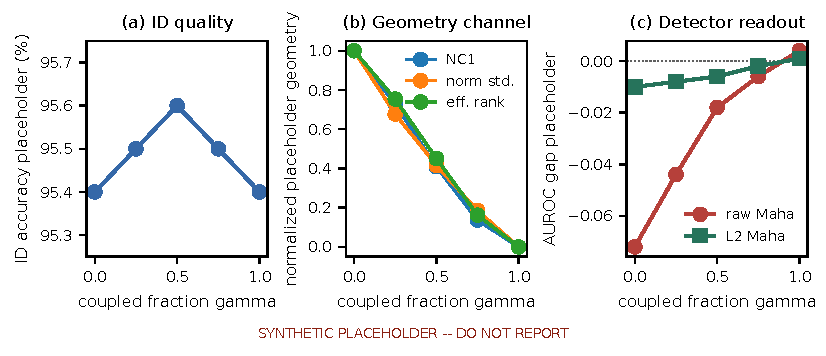
\includegraphics[width=\linewidth]{figures/fig2_wd_coupling_interpolation.pdf}
\caption{SYNTHETIC PLACEHOLDER -- DO NOT REPORT. Placeholder layout for the
AdamW-to-Adam interpolation experiment. The plotted values are synthetic and
must be replaced by measured results. The intended test is whether geometry and
detector behavior move along the weight-decay-coupling axis even when ID
accuracy remains comparable.}
\label{fig:wd-coupling-interpolation}
\end{figure}

\begin{table}[t]
\caption{SYNTHETIC PLACEHOLDER -- DO NOT REPORT. Summary for the
AdamW-to-Adam interpolation. These values are layout placeholders only and must
be replaced by measured results.}
\label{tab:dummy-interpolation-summary}
\begin{center}
\footnotesize
\setlength{\tabcolsep}{5pt}
\renewcommand{\arraystretch}{1.15}
\begin{tabular}{@{}cccccc@{}}
\toprule
\(\gamma\) & ID Acc. & NC1 & Norm std. & Eff. rank & Near AUROC gap \\
\midrule
0.00 & 95.4 & 0.081 & 1.42 & 38.0 & -0.072 \\
0.25 & 95.5 & 0.069 & 1.21 & 34.5 & -0.044 \\
0.50 & 95.6 & 0.055 & 1.04 & 30.2 & -0.018 \\
0.75 & 95.5 & 0.043 & 0.89 & 26.1 & -0.006 \\
1.00 & 95.4 & 0.037 & 0.77 & 23.8 &  0.004 \\
\bottomrule
\end{tabular}
\end{center}
\end{table}


We also compare the size of the coupled-versus-decoupled gap in adaptive and
non-adaptive optimizers. Let
\[
    \Delta_{\mathrm{nonadapt}}
    =
    d\bigl(G_{\mathrm{SGD}},G_{\mathrm{SGDW}}\bigr),
    \qquad
    \Delta_{\mathrm{adapt}}
    =
    d\bigl(G_{\mathrm{Adam}},G_{\mathrm{AdamW}}\bigr),
\]
where \(d(\cdot,\cdot)\) is a standardized distance over the ID geometry
fingerprint. The same comparison is computed for detector-family outputs. If
the adaptive preconditioner amplifies the effect of coupling, then the
Adam--AdamW gap should be larger than the SGD--SGDW gap under matched training
conditions.

\begin{figure}[t]
\centering
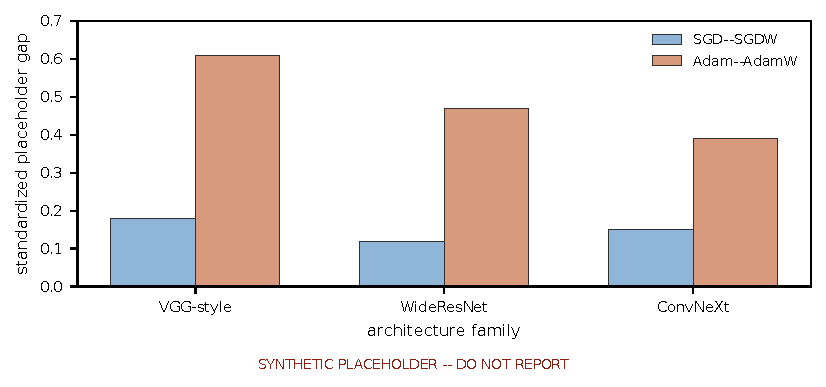
\includegraphics[width=\linewidth]{figures/fig3_adaptive_coupling_gap.pdf}
\caption{SYNTHETIC PLACEHOLDER -- DO NOT REPORT. Placeholder layout for comparing
the Adam--AdamW gap with the SGD--SGDW gap. Values are synthetic placeholders.
The intended figure compares standardized geometry distances and detector-family
distances across architecture families.}
\label{fig:adaptive-coupling-gap}
\end{figure}

If ID accuracy changes strongly along the interpolation, the sweep should be
interpreted as a hyperparameter sensitivity study rather than a clean mechanism
test. If ID accuracy is stable but geometry does not move, then weight-decay
coupling is not the dominant geometry intervention in that setting.

\subsection{Detector Families Respond Through Different Readout Channels}
\label{subsec:detector-readout-channel-response}

We next ask whether detector families inherit optimizer-induced geometry changes
uniformly. The compatibility view predicts that they should not. Logit-based
scores read output confidence and margins; raw Mahalanobis and raw kNN read
radial distance, class separation, and local feature-bank structure;
DDU-style Gaussian feature-density / GMM scores read covariance and density; and
angular or subspace diagnostics read prototype and residual structure.

Figure~\ref{fig:detector-family-delta-heatmap} reports the planned
optimizer-relative AUROC gap heatmap. The reference is the matched SGD anchor
within each architecture and dataset. Positive values indicate that the detector
family improves relative to the anchor, and negative values indicate
degradation. The purpose of this figure is not to declare a winning optimizer.
The purpose is to show whether the same representation remains compatible with
some readouts while becoming less compatible with others.

\begin{figure}[t]
\centering
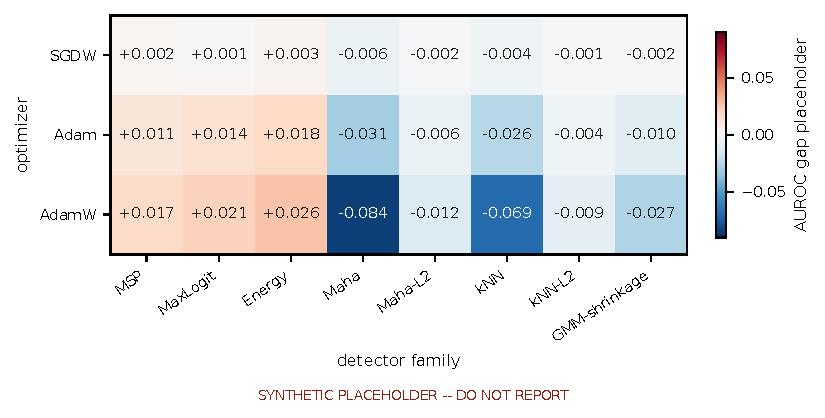
\includegraphics[width=\linewidth]{figures/fig4_detector_family_delta_heatmap.pdf}
\caption{SYNTHETIC PLACEHOLDER -- DO NOT REPORT. Placeholder detector-family
AUROC gap heatmap. Values are synthetic placeholders. The intended result format
compares logit, raw distance, L2 distance, Gaussian density, angular, and
subspace readouts relative to a matched SGD anchor.}
\label{fig:detector-family-delta-heatmap}
\end{figure}

A useful diagnostic pattern is a split between logit and feature readouts. If
logit scores remain stable while raw feature-distance scores degrade, the
optimizer has not produced a uniformly worse model. Instead, it has produced a
representation that is less compatible with the raw distance channel. If all
detectors degrade together, the result is more likely to reflect a broad model
quality issue rather than a geometry--detector compatibility effect.

\subsection{Diagnostic Controls Localize Geometry Channels}
\label{subsec:diagnostic-controls-localize-channels}

We then use detector-side controls to localize which geometry channel carries a
detector gap. These controls are diagnostic interventions, not proposed universal
fixes. L2 normalization removes the radial feature-norm channel; tied, diagonal,
and shrinkage covariance variants probe covariance estimation and conditioning;
and PCA or residual-subspace diagnostics separate principal ID directions from
residual directions.

The radial-channel diagnostic compares raw Mahalanobis and raw kNN against their
L2-normalized counterparts using the same checkpoints, ID feature bank, OOD
datasets, and score direction convention. Recovery after L2 normalization
indicates that the raw detector gap is carried by radial or norm-coupled
geometry.

\begin{figure}[t]
\centering
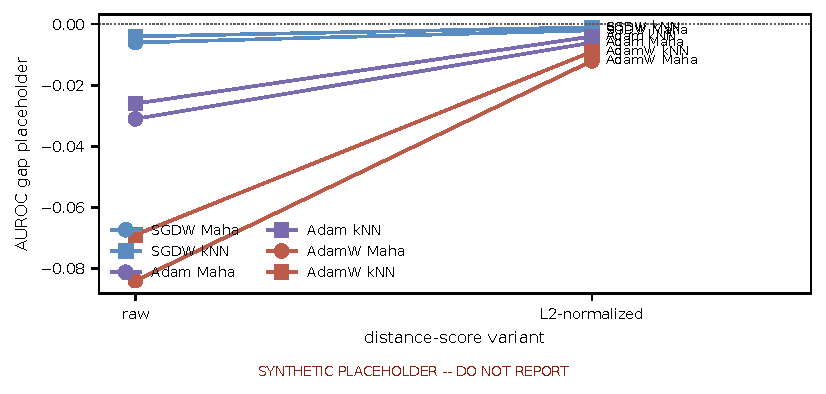
\includegraphics[width=\linewidth]{figures/fig5_l2_recovery_paths.pdf}
\caption{SYNTHETIC PLACEHOLDER -- DO NOT REPORT. Placeholder raw-to-L2 recovery
plot for Mahalanobis and kNN. Values are synthetic placeholders. Strong movement
toward zero after L2 normalization would implicate a radial or norm-coupled
failure channel.}
\label{fig:l2-recovery-paths}
\end{figure}

Covariance controls test a different failure mode. Mahalanobis-style and
DDU-style Gaussian feature-density / GMM readouts depend on inverse covariance,
covariance volume, and the stability of covariance estimates. We therefore
compare full, tied, diagonal, shrinkage, and PCA-projected covariance variants.
If shrinkage or diagonalization reduces the detector gap, the failure likely
involves unstable covariance estimation or ill-conditioning. If PCA projection
helps while shrinkage does not, the mismatch may be concentrated in nuisance or
residual directions.

\begin{table}[t]
\caption{SYNTHETIC PLACEHOLDER -- DO NOT REPORT. Covariance-control results.
Values are AUROC gaps relative to a matched SGD anchor and are not experimental
evidence.}
\label{tab:dummy-covariance-controls}
\begin{center}
\footnotesize
\setlength{\tabcolsep}{5pt}
\renewcommand{\arraystretch}{1.15}
\begin{tabular}{@{}lrrrrr@{}}
\toprule
Optimizer & Full GMM & Tied GMM & Diag. GMM & Shrinkage GMM & PCA-GMM \\
\midrule
SGDW  & -0.006 & -0.004 & -0.003 & -0.002 &  0.001 \\
Adam  & -0.018 & -0.014 & -0.010 & -0.006 & -0.004 \\
AdamW & -0.061 & -0.052 & -0.033 & -0.027 & -0.019 \\
\bottomrule
\end{tabular}
\end{center}
\end{table}


Angular, prototype, and subspace diagnostics are included when their score
conventions are fixed. The planned analysis compares NC alignment, class-mean
angular structure, classifier--feature alignment, effective rank, PCA explained
variance, and residual energy against CTM-style, NECO-style, prototype-cosine,
and residual-subspace scores. If these diagnostics do not follow NC or subspace
measurements, the score convention, PCA dimension, class-selection rule, or
implementation should be checked before interpreting the result as a failure of
the framework.

\begin{figure}[t]
\centering
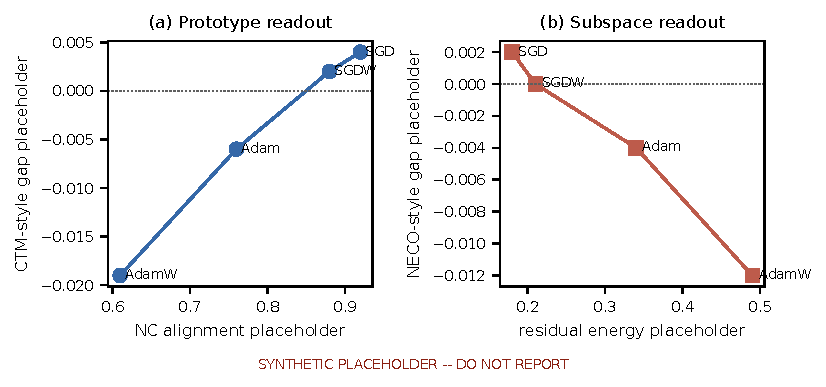
\includegraphics[width=\linewidth]{figures/fig6_prototype_subspace_alignment.pdf}
\caption{SYNTHETIC PLACEHOLDER -- DO NOT REPORT. Placeholder prototype/subspace
diagnostic plot. Values are synthetic placeholders. The intended analysis relates
NC alignment, effective rank, and residual energy to CTM-style, NECO-style,
prototype, and residual-subspace readouts.}
\label{fig:prototype-subspace-alignment}
\end{figure}

Together, the radial, covariance, and subspace controls test whether detector
failures are explained by specific geometry channels or whether they reflect a
broader representation mismatch.

\subsection{Geometry Fingerprints as Detector Diagnostics}
\label{subsec:geometry-fingerprints-detector-diagnostics}

Finally, we ask whether ID-only geometry can guide detector diagnostics before
using OOD validation data. This is a diagnostic goal rather than a claim that ID
geometry fully determines OOD performance. The simplest version is a rule-based
selector: high norm dispersion recommends L2-based controls, poor covariance
conditioning recommends shrinkage or diagonal covariance, strong NC alignment
recommends angular or prototype diagnostics, and large residual energy
recommends PCA or residual-subspace probes.

\begin{table}[t]
\caption{SYNTHETIC PLACEHOLDER -- DO NOT REPORT. Geometry-aware diagnostic
selector. The rules and values are illustrative placeholders only.}
\label{tab:dummy-geometry-selector}
\begin{center}
\footnotesize
\setlength{\tabcolsep}{4pt}
\renewcommand{\arraystretch}{1.15}
\begin{tabular}{@{}p{0.25\textwidth}p{0.26\textwidth}p{0.30\textwidth}p{0.10\textwidth}@{}}
\toprule
ID geometry signal & Suggested diagnostic & Expected compatible family & Dummy hit rate \\
\midrule
High norm dispersion & L2 normalization & L2-Mahalanobis, L2-kNN & 0.78 \\
High covariance condition & Shrinkage / diagonal covariance & GMM, Mahalanobis & 0.71 \\
Strong NC alignment & Angular / prototype readout & CTM-style, prototype cosine & 0.69 \\
High residual energy & PCA / residual probe & NECO-style, PCA residual & 0.64 \\
Mixed geometry profile & Evaluate multiple controls & No single-family recommendation & 0.52 \\
\bottomrule
\end{tabular}
\end{center}
\end{table}


A learned selector can be evaluated after enough architecture--optimizer--seed
cells are available. The target should not be the single best detector on one OOD
dataset. A more stable target is a detector family or control type that remains
competitive across OOD regimes. If the selector fails, then either the fingerprint
\(G(h,W)\) is missing important geometry channels, or OOD severity information is
necessary to choose a detector reliably.

The experiments therefore test both links in the optimizer--geometry--detector
pathway. The interpolation and paired optimizer comparisons test whether
optimizer choice moves the predicted ID geometry channels. The detector-family
and diagnostic-control analyses test whether downstream scores respond according
to their readout channel. The geometry-aware diagnostic analysis tests whether
the same ID fingerprint can be useful before OOD validation.


\section{Discussion}
\label{sec:discussion}
\subsection{Compatibility, Not Optimizer Ranking}
\label{subsec:compatibility-not-ranking}

The central message of this paper is not that one optimizer is universally better
for uncertainty estimation. The relevant object is the compatibility between the
geometry induced by the optimizer and the geometry read by the detector. An
optimizer can produce a representation that remains favorable for logit-based
scores while changing feature-space properties that are important for distance,
density, neighborhood, angular, or subspace readouts. Conversely, a detector that
works well under one optimizer-induced geometry may become less reliable when the
same model family is trained with a different update rule.

This view changes how optimizer improvements should be evaluated. Accuracy,
calibration, or logit-level OOD behavior do not by themselves certify
feature-based uncertainty. When downstream reliability depends on penultimate
features, the optimizer should be evaluated together with the representation
geometry it induces and the detector family that will read that geometry. This is
especially important when comparing coupled and decoupled weight decay or
adaptive and non-adaptive optimizers, because these choices can alter class
structure, feature norms, covariance spectra, and local feature-bank geometry
without necessarily producing a large change in ID accuracy.

The compatibility view also avoids an overly broad conclusion. If a detector gap
appears under one optimizer, this does not imply that the optimizer is globally
bad or that the detector is intrinsically weak. It indicates that the detector's
readout channel and the learned geometry may be mismatched. The goal is therefore
to identify which geometry channel carries the mismatch and whether a diagnostic
control can localize it.

\subsection{What the Diagnostics Can and Cannot Identify}
\label{subsec:what-diagnostics-identify}

The diagnostic interventions in this work are not proposed as new OOD detectors
or universal fixes. Their role is to perturb or stabilize a specific geometry
channel so that detector behavior can be interpreted more mechanistically. L2
normalization removes radial feature-norm variation before distance-based
scoring. Covariance controls such as tied, diagonal, and shrinkage estimates
alter the conditioning and precision structure used by Mahalanobis-style and
DDU-style Gaussian feature-density scores. PCA and residual-subspace diagnostics
separate principal ID structure from directions that may contain nuisance or
shift-related variation.

A recovery after a diagnostic intervention narrows the set of plausible failure
channels, but it does not prove a complete causal mechanism by itself. For
example, if raw Mahalanobis or raw kNN improves after L2 normalization, radial or
norm-coupled geometry is implicated. However, the remaining behavior may still
depend on class separation, covariance anisotropy, local density, or OOD
severity. Similarly, if shrinkage improves a Gaussian density score, covariance
estimation or conditioning is involved; if the gap remains, covariance correction
alone is not sufficient to explain the mismatch.

The strongest evidence for the proposed framework would therefore come from an
aligned pattern across multiple measurements: optimizer choice changes the ID
geometry fingerprint, detector families respond according to their readout
channels, and diagnostic controls remove or reduce the corresponding failure
mode. A single geometry metric or a single detector ablation should not be
overinterpreted as a complete explanation.

\subsection{Limitations and Scope}
\label{subsec:limitations-scope}

This study is intentionally controlled. Its purpose is to test the
optimizer--geometry--detector pathway, not to provide an exhaustive benchmark
over all OOD detectors, architectures, datasets, or training recipes. The main
claims should therefore be limited to the evaluated optimizer families,
architectures, datasets, and detector implementations. Broader datasets,
larger-scale models, pretrained regimes, and additional OOD shifts are important
settings for testing how far the compatibility view generalizes.

The comparisons should also be interpreted as accuracy-controlled rather than
perfectly accuracy-matched. Residual differences in ID accuracy, calibration,
training stability, or hyperparameter sensitivity may contribute to detector
behavior and should be reported alongside geometry and OOD metrics. In
particular, if the AdamW-to-Adam interpolation changes ID accuracy strongly, it
should be interpreted as a joint optimization-and-geometry effect rather than a
clean geometry intervention.

Detector coverage is another limitation. DDU-style Gaussian feature-density
scores in this paper refer to the post-hoc Gaussian density scoring component,
not necessarily a faithful reproduction of the original DDU training recipe.
Likewise, CTM-, NECO-, prototype-, and residual-subspace diagnostics should be
treated as extended probes unless their score conventions, PCA dimensions,
class-selection rules, and implementation details are fixed within the same
evaluation protocol.

Finally, the geometry--detector link studied here is diagnostic rather than a
complete causal proof. Stronger causal claims would require direct interventions
that change one geometry channel while holding others fixed, tighter ID-accuracy
bands, and broader architecture--dataset coverage. The contribution of this
paper is to make the optimizer-induced geometry pathway explicit and to provide a
testable diagnostic structure for evaluating feature-based uncertainty.


\section{Conclusion}
\label{sec:conclusion}
We studied optimizer choice as a geometry intervention for feature-based
uncertainty. In an accuracy-controlled selected-configuration study with SGD,
Adam, and AdamW, we find that comparable ID performance can hide substantial
differences in penultimate representation geometry and detector-family behavior.
Selected optimizers induce different fingerprints in neural-collapse geometry, feature
norms, within-class dispersion, and class separation, and detector families read
these fingerprints differently.

The clearest example is the AdamW-selected raw-distance split. These
configurations can remain competitive under logit-based readouts while showing
large near-OOD gaps under raw Mahalanobis and kNN. L2 normalization recovers much
of this gap, implicating a radial or norm-coupled failure channel, whereas
covariance shrinkage has a more limited and detector-dependent effect. These
results support a compatibility view rather than an optimizer-good/bad ranking.

The key lesson is that optimizer, penultimate representation geometry, and
detector readout should be evaluated jointly. Feature-based uncertainty should
therefore be evaluated as a geometry--detector compatibility problem, not as an
accuracy-only model-selection problem.


\bibliography{references}
\bibliographystyle{iclr2026_conference}

\appendix
\section{Full Geometry Metric Definitions}
\label{app:geometry-metrics}
This appendix gives the full definitions of the geometry metrics used in the
main text. The main paper groups these metrics by geometry channel: class
structure, radial norm geometry, covariance spectrum, local density, and
subspace structure. These metrics are not treated as competing explanations in
isolation; they are complementary fingerprints of the penultimate
representation.

\subsection{Class Structure and Neural Collapse Metrics}
\label{app:class-structure-nc}

Let \(\mu_c\) denote the class mean of ID training features and let
\[
    \bar{\mu}
    =
    \frac{1}{K}\sum_{c=1}^{K}\mu_c,
    \qquad
    \tilde{\mu}_c
    =
    \mu_c-\bar{\mu}.
\]
For class \(c\), let \(\Sigma_c\) be the class covariance and let
\[
    \Sigma_W
    =
    \frac{1}{K}\sum_{c=1}^{K}\Sigma_c
\]
be the pooled within-class covariance. The between-class covariance is
\[
    \Sigma_B
    =
    \frac{1}{K}\sum_{c=1}^{K}
    \tilde{\mu}_c \tilde{\mu}_c^\top .
\]
A standard NC1-style diagnostic is
\[
    \mathrm{NC1}
    =
    \frac{1}{K}\operatorname{tr}
    \left(\Sigma_W \Sigma_B^\dagger\right),
\]
where \(\dagger\) denotes the Moore--Penrose pseudoinverse. Smaller values
indicate stronger within-class collapse relative to between-class variation.

NC2 measures the angular structure of the centered class means
\(\{\tilde{\mu}_c\}_{c=1}^K\), typically by comparing their normalized Gram
matrix to the simplex ETF target. NC3 measures the alignment between classifier
weights \(w_c\) and centered class means \(\tilde{\mu}_c\). This is the class
structure channel most directly connected to CTM classifier-feature cosine
scores. We also report direct summaries such as WithinVar, the average
within-class dispersion, and InterDist, the average distance between class
means.

\subsection{Radial Norm Statistics}
\label{app:radial-norm-statistics}

We decompose each feature into norm and direction:
\[
    f_\theta(x)=r(x)u(x),
    \qquad
    r(x)=\|f_\theta(x)\|_2,
    \qquad
    \|u(x)\|_2=1.
\]
We measure the mean, standard deviation, quantiles, and class-wise dispersion of
\(r(x)\). These statistics test whether an optimizer changes feature magnitude
globally, by class, or by sample. Radial geometry can affect MaxLogit, Energy,
Mahalanobis, kNN, and GMM scores. Cosine-based scores such as CTM are
invariant to feature norm, and NeCo projection ratios normalize by the
feature norm.

\subsection{Covariance Spectrum and Conditioning}
\label{app:covariance-spectrum-conditioning}

For each class covariance, we consider the eigendecomposition
\[
    \Sigma_c
    =
    U_c
    \operatorname{diag}(\lambda_{c,1},\ldots,\lambda_{c,d})
    U_c^\top .
\]
We summarize the covariance spectrum by trace, leading eigenvalue, anisotropy,
effective rank, condition number, and cumulative explained variance. These
metrics test whether an optimizer spreads features unevenly across directions,
creates ill-conditioned covariance estimates, or changes the stability of
inverse-covariance detectors.

\subsection{Local Density Diagnostics}
\label{app:local-density-diagnostics}

kNN detectors do not assume a Gaussian covariance model. They read local
neighborhood spacing in the ID feature bank. Let
\[
    d_k(f_\theta(x),\mathcal{F}_{\mathrm{tr}})
\]
denote the distance from \(f_\theta(x)\) to its \(k\)-th nearest neighbor in the
training feature bank \(\mathcal{F}_{\mathrm{tr}}\). We compare the
distributions of this distance for ID and OOD samples. When feature labels are
available, we can additionally separate same-class and cross-class
nearest-neighbor distances for ID data. This reveals whether an optimizer
changes within-class local density or boundary-neighborhood geometry.

\subsection{Subspace Diagnostics}
\label{app:subspace-diagnostics}

Subspace-aware scores such as NeCo and PCA reconstruction error read whether a
feature lies in the principal ID subspace. Let \(P\in\mathbb{R}^{d\times r}\)
contain the top \(r\) principal directions of the ID training features. Then
\(PP^\top\) is the projection matrix onto the selected ID subspace. We measure
retained dimension, explained variance, projection norm, and residual norm:
\[
    \|P^\top f_\theta(x)\|_2,
    \qquad
    \|(I-PP^\top)f_\theta(x)\|_2.
\]
These quantities test whether an optimizer keeps ID features in a compact,
task-relevant subspace or spreads them into residual directions.


\section{Detector Score Definitions and Score Direction}
\label{app:detector-scores}
All detector scores are converted to a higher-is-ID-like convention before
computing AUROC, AUPR-IN, and FPR95. This appendix lists the score definitions
used in the experiments and records whether each score is a faithful
reproduction of an existing method or a diagnostic variant used to probe a
geometry channel.

\subsection{Logit-Based Scores}
\label{app:logit-based-scores}

Logit-based detectors read output confidence, logit scale, and margin structure.
The maximum softmax probability score is
\[
    S_{\mathrm{MSP}}(x)
    =
    \max_c p_\theta(y=c\mid x).
\]
The Energy score is written in the higher-is-ID-like direction used in this
paper:
\[
    S_{\mathrm{Energy}}(x)
    =
    T\log\sum_{c=1}^{K}\exp(z_c(x)/T).
\]
The MaxLogit score is
\[
    S_{\mathrm{MaxLogit}}(x)
    =
    \max_c z_c(x).
\]
When negative entropy is reported, it is also oriented so larger values are more
ID-like.

\subsection{Distance-Based Feature Scores}
\label{app:distance-based-feature-scores}

The Mahalanobis detector reads class means and tied covariance through a
precision-weighted distance:
\[
    S_{\mathrm{Maha}}(x)
    =
    -\min_c
    (f_\theta(x)-\mu_c)^\top
    \Sigma_W^{-1}
    (f_\theta(x)-\mu_c).
\]
The negative sign enforces the higher-is-ID-like score convention. A
Mahalanobis-L2 variant applies the same score after normalizing features to unit
norm.

kNN detectors read local neighborhood distance in the ID training feature bank:
\[
    S_{\mathrm{kNN}}(x)
    =
    -d_k(f_\theta(x),\mathcal{F}_{\mathrm{tr}}),
\]
where \(d_k\) is the \(k\)-th nearest-neighbor distance. L2-kNN applies the same
score after feature normalization, allowing us to test whether the
local-distance detector depends on radial scale.

\subsection{Gaussian Feature-Density Scores}
\label{app:gaussian-feature-density-scores}

Gaussian feature-density detectors score a feature by a
class-conditional mixture likelihood:
\[
    S_{\mathrm{GMM}}(x)
    =
    \log \sum_{c=1}^{K}
    \pi_c
    \mathcal{N}(f_\theta(x)\mid \mu_c,\Sigma_c).
\]
We distinguish tied, diagonal, and shrinkage covariance variants as diagnostic
controls for covariance estimation and covariance conditioning.

We use Gaussian feature-density score to refer to the density scoring component
inspired by DDU. We do not claim to reproduce
the full original DDU training recipe unless spectral normalization and the
associated training protocol are explicitly used. This distinction is important
because spectral normalization is itself a training-time geometric regularizer
and can modify the optimizer-induced geometry that this paper aims to measure.

\subsection{Prototype, Angular, and Subspace Scores}
\label{app:prototype-angular-subspace-scores}

The reported results include NCC, prototype-cosine, and ViM diagnostics.
These are useful representation diagnostics but should not be relabeled as CTM
or NeCo.

CTM uses cosine similarity between features and classifier weights:
\[
    S_{\mathrm{CTM}}(x)
    =
    \max_c \cos(w_c,f_\theta(x))
    =
    \max_c
    \frac{w_c^\top f_\theta(x)}
    {\|w_c\|_2\|f_\theta(x)\|_2}.
\]
CTM reads angular alignment rather than feature norm and is directly connected
to NC3 self-duality between classifier weights and class means. In this
draft, CTM is a planned probe rather than an available main result.

NeCo uses the relationship between test features and the principal ID subspace.
With \(P\in\mathbb{R}^{d\times r}\) denoting the matrix of top ID principal
directions, the normalized projection score is
\[
    S_{\mathrm{NeCo}}(x)
    =
    \frac{\|P^\top f_\theta(x)\|_2}
    {\|f_\theta(x)\|_2}.
\]
When using NeCo, we distinguish the official score and fixed PCA configuration
from project-specific simplified variants. Temporary simplified scores are not
used as main results unless their formula, dimension, direction, and
normalization are fixed.

\subsection{Score Direction and Aggregation Convention}
\label{app:score-direction-aggregation}

All scores are oriented so larger values indicate more ID-like inputs before
AUROC, AUPR-IN, and FPR95 are computed. Aggregated near/far tables average over
the OOD datasets in the corresponding group after applying this score direction
convention.


\section{Diagnostic Intervention Details}
\label{app:diagnostic-interventions}
The interventions in this appendix are diagnostic controls rather than proposed
universal fixes. Each intervention removes or stabilizes one geometry channel so
that detector behavior can be interpreted more mechanistically.

\subsection{L2 Normalization}
\label{app:l2-normalization}

Feature normalization removes radial scale:
\[
    \hat{f}_\theta(x)
    =
    \frac{f_\theta(x)}
    {\|f_\theta(x)\|_2+\epsilon}.
\]
Raw and L2-normalized detectors are compared under the same optimizer, dataset,
OOD split, and seed. If raw Mahalanobis or raw kNN performs poorly for one
optimizer but recovers after L2 normalization, the failure includes a
norm-driven component. If a gap remains after L2 normalization, radial scale is
not sufficient to explain the detector behavior.

\subsection{Covariance Shrinkage}
\label{app:covariance-shrinkage}

For class covariance \(\Sigma_c\), shrinkage uses
\[
    \Sigma_{c,\alpha}
    =
    (1-\alpha)\Sigma_c
    +
    \alpha\frac{\operatorname{tr}(\Sigma_c)}{d}I.
\]
This stabilizes inverse covariance by increasing small eigenvalues and pulling
large eigenvalues toward the mean. Tied, diagonal, and shrinkage covariance
variants are treated as diagnostic controls. If GMM or Mahalanobis scores
recover after shrinkage, covariance estimation or covariance conditioning
contributes to the detector behavior.

\subsection{PCA Projection and Residual Diagnostics}
\label{app:pca-projection-residual}

PCA projection preserves the ID principal subspace:
\[
    \hat{f}_\theta(x)
    =
    PP^\top(f_\theta(x)-\mu)+\mu.
\]
A PCA reconstruction-error style score reads the residual component:
\[
    S_{\mathrm{PCARec}}(x)
    =
    -\|(I-PP^\top)(f_\theta(x)-\mu)\|_2.
\]
The negative sign follows the higher-is-ID-like convention. These diagnostics
test whether optimizer-induced geometry differences concentrate inside the ID
principal subspace or in residual directions. The PCA fitting split, retained
dimension rule, and score direction should be fixed before reporting PCA or
NeCo scores as main results.

\subsection{Angular Alignment Probes}
\label{app:angular-alignment-probes}

CTM is an angular alignment probe because it removes feature norm and reads
cosine similarity between classifier weights and features. It should be compared
with NC3 classifier-mean alignment rather than interpreted as a generic
feature-distance score. CTM is reported in the main text only when the official
score convention and implementation are fixed for the experiment package.

\subsection{Implementation Notes and Score Convention}
\label{app:diagnostic-implementation-notes}

Diagnostic controls should use the same training checkpoints, feature extraction
layer, ID split, OOD datasets, and score direction convention as the corresponding
raw detector. Manual post-hoc variants should be labeled explicitly as
diagnostics. They should not be presented as faithful reproductions of methods
whose original training recipe includes additional regularizers or architectural
constraints.


\section{Statistical Summary Details}
\label{app:statistical-summaries}
This appendix describes the statistical summaries used to aggregate detector and
geometry measurements. The main text focuses on optimizer-induced gaps, while
the appendix reports seed variability, full detector tables, and secondary
robustness summaries.

\subsection{Seed Means and Standard Deviations}
\label{app:seed-means-std}

For each optimizer \(o\), detector \(m\), OOD dataset \(q\), and seed \(s\), we
compute AUROC, AUPR-IN, and FPR95. Main tables report seed means and standard
deviations. For a metric value \(A_{o,m,q,s}\), the seed mean is
\[
    \overline{A}_{o,m,q}
    =
    \frac{1}{S}\sum_{s=1}^{S}A_{o,m,q,s}.
\]
The same aggregation is used for ID accuracy, calibration metrics, and geometry
metrics when seed-level values are available.

\subsection{Paired Optimizer Gaps}
\label{app:paired-optimizer-gaps}

To isolate optimizer effects, we define paired detector gaps relative to the SGD
reference under the same dataset, detector, and seed:
\[
    \Delta^{\mathrm{det}}_{o,m,q,s}
    =
    A_{o,m,q,s}
    -
    A_{\mathrm{SGD},m,q,s}.
\]
For selected configurations, we also report seed-averaged gaps:
\[
    \Delta^{\mathrm{det}}_{o,m,q}
    =
    \overline{A}_{o,m,q}
    -
    \overline{A}_{\mathrm{SGD},m,q}.
\]
For a geometry metric \(G_g\), the corresponding geometry gap is
\[
    \Delta^{\mathrm{geo}}_{o,g}
    =
    G_{o,g}
    -
    G_{\mathrm{SGD},g}.
\]
The purpose of this analysis is to test whether optimizer-induced geometry gaps
move consistently with detector-family gaps.

\subsection{Family-Level Rank Summaries}
\label{app:family-rank-summaries}

When several detectors perform similarly, a single winning detector can be
misleading. Family-level rank summaries compare average ranks across
logit-based, covariance-based, local-neighborhood, angular-alignment, and
subspace detector families. When needed, a rank-based comparison can report
detector families that are statistically competitive with the best score. This
analysis is secondary; it prevents single-winner overinterpretation rather than
serving as the main contribution.

\subsection{Geometry--Detector Association Checks}
\label{app:geometry-detector-association}

As a secondary analysis, we can compare distances between optimizer geometry
fingerprints and distances between detector response vectors. Let \(G_o\) denote
the geometry vector for optimizer \(o\), and let \(R_o\) denote its detector
response vector. We compute
\[
    D^{\mathrm{geo}}_{o,o'}
    =
    d(G_o,G_{o'}),
    \qquad
    D^{\mathrm{det}}_{o,o'}
    =
    d(R_o,R_{o'}).
\]
If the two distance matrices vary together, optimizers that produce similar
geometry also tend to produce similar detector behavior. This is an association
check, not a causal proof.

\subsection{Interpretation Limits}
\label{app:statistical-interpretation-limits}

Family-level rank summaries and geometry--detector association checks are
secondary analyses. They are used to avoid overinterpreting a single detector
winner, not to establish a causal relationship between a geometry metric and
detector performance. Causal interpretation still depends on controlled
optimizer comparisons, diagnostic interventions, and additional robustness
experiments.


\section{Additional Experimental Details}
\label{app:experimental-details}
This appendix reports the experimental coverage and numerical tables supporting
Section~\ref{sec:experiments}. The main text summarizes the controlled
CIFAR-10/WideResNet-28-10 study, while this appendix records the run inventory,
available detector families, OOD coverage, and full aggregate tables.

\subsection{Reported Coverage and Result Inventory}
\label{app:reported-coverage-inventory}

Table~\ref{tab:experiment-inventory} summarizes the reported experimental
coverage and planned extensions. The distinction is included for reproducibility:
main-text claims use only the reported CIFAR-10/WideResNet-28-10 setting, while
additional planned coverage is treated as future robustness evidence.

\begin{table}[t]
\caption{Reported experimental coverage and planned extensions. Main-text claims
use the reported CIFAR-10/WideResNet-28-10 selected-configuration setting;
additional coverage is listed as robustness evidence for future versions.}
\label{tab:experiment-inventory}
\begin{center}
\small
\setlength{\tabcolsep}{4pt}
\renewcommand{\arraystretch}{1.12}
\begin{tabular}{@{}>{\raggedright\arraybackslash}p{0.17\textwidth}>{\raggedright\arraybackslash}p{0.35\textwidth}>{\raggedright\arraybackslash}p{0.28\textwidth}>{\raggedright\arraybackslash}p{0.13\textwidth}@{}}
\toprule
Component & Reported coverage & Additional planned coverage & Role \\
\midrule
ID setting
& CIFAR-10 with train/validation/test split metadata.
& CIFAR-100 ID comparison.
& Main setting; robustness extension \\
Backbone
& WideResNet-28-10 with dropout 0.3, evaluated at 350 epochs.
& Additional backbones such as ResNet or VGG.
& Main setting; appendix or future \\
Optimizers
& Five selected configurations: two SGD, one Adam, two AdamW; seeds 0, 1, 2.
& Tighter accuracy matching and local LR/WD grids.
& Main caveat \\
OOD datasets
& CIFAR-100 and TinyImageNet as near-OOD; SVHN and MNIST as far/easy-far controls.
& Textures and Places365.
& Main setting; coverage extension \\
Detectors
& MSP, MaxLogit, Energy, negative entropy, Mahalanobis, L2-Mahalanobis, kNN, L2-kNN, and GMM tied/diagonal/shrinkage scores.
& CTM and NeCo probes once score conventions and implementations are fixed.
& Main setting; planned probes \\
Geometry
& NC1, NC3 alignment, WithinVar, InterDist, feature-norm statistics, anisotropy, effective rank, clipped condition number, and raw covariance eigenspectra.
& Local-density summaries and official subspace probes.
& Main setting; planned diagnostics \\
\bottomrule
\end{tabular}
\end{center}
\end{table}


\subsection{Full Geometry Tables}
\label{app:full-geometry-tables}

The main text discusses standardized geometry fingerprints at the level of
geometry channels. Table~\ref{tab:geometry-fingerprint} reports the corresponding
numerical values for each selected optimizer configuration.

\begin{table}[t]
\caption{Geometry fingerprints for the selected configurations. Geometry metrics
are computed on the ID training split unless otherwise stated; values are seed
mean $\pm$ standard deviation.}
\label{tab:geometry-fingerprint}
\begin{center}
\scriptsize
\setlength{\tabcolsep}{3pt}
\renewcommand{\arraystretch}{1.08}
\resizebox{\linewidth}{!}{%
\begin{tabular}{@{}lcccccccc@{}}
\toprule
Configuration & Test acc. (\%) & NC1 \(\downarrow\) & NC3 \(\uparrow\) & InterDist \(\uparrow\) & WithinVar & Norm mean & Norm std. & Eff. rank \\
\midrule
SGD, wd \(5{\times}10^{-4}\) & 95.83 $\pm$ 0.16 & 0.051 $\pm$ 0.002 & 0.950 $\pm$ 0.003 & 16.62 $\pm$ 0.19 & 18.61 $\pm$ 0.99 & 14.23 $\pm$ 0.15 & 1.79 $\pm$ 0.06 & 59.55 $\pm$ 1.80 \\
SGD, wd \(2{\times}10^{-4}\) & 95.58 $\pm$ 0.14 & 0.067 $\pm$ 0.002 & 0.938 $\pm$ 0.001 & 14.28 $\pm$ 0.17 & 17.52 $\pm$ 0.34 & 12.88 $\pm$ 0.13 & 1.74 $\pm$ 0.01 & 57.92 $\pm$ 1.09 \\
Adam & 94.49 $\pm$ 0.10 & 0.190 $\pm$ 0.002 & 0.905 $\pm$ 0.002 & 13.34 $\pm$ 0.08 & 23.86 $\pm$ 0.34 & 14.39 $\pm$ 0.12 & 2.03 $\pm$ 0.07 & 25.55 $\pm$ 0.39 \\
AdamW, wd \(1{\times}10^{-4}\) & 94.47 $\pm$ 0.24 & 0.277 $\pm$ 0.006 & 0.613 $\pm$ 0.005 & 5.23 $\pm$ 0.13 & 10.08 $\pm$ 0.28 & 6.21 $\pm$ 0.09 & 1.32 $\pm$ 0.04 & 76.92 $\pm$ 6.07 \\
AdamW, wd \(5{\times}10^{-4}\) & 94.36 $\pm$ 0.02 & 0.269 $\pm$ 0.008 & 0.615 $\pm$ 0.005 & 5.47 $\pm$ 0.07 & 10.62 $\pm$ 0.51 & 6.50 $\pm$ 0.07 & 1.38 $\pm$ 0.03 & 74.15 $\pm$ 3.60 \\
\bottomrule
\end{tabular}}
\end{center}
\end{table}


\subsection{Full OOD Results}
\label{app:full-ood-results}

The main text emphasizes optimizer-induced detector response gaps.
Table~\ref{tab:detector-family-auroc} reports the aggregate AUROC values behind that
discussion, averaged within the reported near-OOD and far/easy-far groups. All
scores follow the higher-is-ID-like convention described in
Appendix~\ref{app:score-direction-aggregation}.

\begin{table}[t]
\caption{Detector-family AUROC under the reported OOD coverage. Entries are seed
means averaged within the indicated OOD regime. Near-OOD uses CIFAR-100 and
TinyImageNet; far/easy-far uses SVHN and MNIST.}
\label{tab:detector-family-auroc}
\begin{center}
\small
\setlength{\tabcolsep}{5pt}
\renewcommand{\arraystretch}{1.08}
\begin{tabular}{@{}lcccccc@{}}
\toprule
Configuration & Logit & Maha & Maha-L2 & kNN & kNN-L2 & GMM-shr. \\
\midrule
\multicolumn{7}{@{}l}{\emph{Near-OOD AUROC}} \\
SGD, wd \(5{\times}10^{-4}\) & 0.855 & 0.867 & 0.886 & 0.903 & 0.903 & 0.907 \\
SGD, wd \(2{\times}10^{-4}\) & 0.845 & 0.860 & 0.870 & 0.903 & 0.902 & 0.905 \\
Adam & 0.900 & 0.568 & 0.728 & 0.849 & 0.881 & 0.804 \\
AdamW, wd \(1{\times}10^{-4}\) & 0.900 & 0.416 & 0.856 & 0.568 & 0.890 & 0.793 \\
AdamW, wd \(5{\times}10^{-4}\) & 0.901 & 0.418 & 0.855 & 0.590 & 0.888 & 0.796 \\
\midrule
\multicolumn{7}{@{}l}{\emph{Far/easy-far AUROC}} \\
SGD, wd \(5{\times}10^{-4}\) & 0.939 & 0.974 & 0.984 & 0.937 & 0.955 & 0.957 \\
SGD, wd \(2{\times}10^{-4}\) & 0.933 & 0.963 & 0.982 & 0.935 & 0.952 & 0.946 \\
Adam & 0.920 & 0.635 & 0.917 & 0.881 & 0.911 & 0.737 \\
AdamW, wd \(1{\times}10^{-4}\) & 0.922 & 0.541 & 0.988 & 0.674 & 0.988 & 0.758 \\
AdamW, wd \(5{\times}10^{-4}\) & 0.900 & 0.610 & 0.992 & 0.762 & 0.991 & 0.782 \\
\bottomrule
\end{tabular}
\end{center}
\end{table}


\subsection{Additional Tables}
\label{app:additional-tables}

Per-dataset AUROC, AUPR-IN, and FPR95 tables can be generated from the processed
summary directory \texttt{results/processed/wrn350\_selected\_3seed\_20260612/}.
The relevant source files are \texttt{ood\_by\_dataset\_long.csv},
\texttt{mean\_std.csv}, and \texttt{paired\_delta.csv}.

\subsection{Diagnostic Gap Summary}
\label{app:diagnostic-gap-summary}

Table~\ref{tab:diagnostic-gap-summary} reports paired diagnostic gaps for the
AdamW, weight decay \(1{\times}10^{-4}\), selected configuration relative to the
SGD anchor on near-OOD AUROC.

\begin{table}[h!]
\caption{Example diagnostic gaps for AdamW, wd \(1{\times}10^{-4}\), relative to
the SGD, wd \(5{\times}10^{-4}\), anchor on near-OOD AUROC. Values are paired
seed mean $\pm$ standard deviation. The large reduction from raw to L2-normalized
feature scores is descriptive evidence for a radial or norm-coupled failure
channel, not a complete causal proof.}
\label{tab:diagnostic-gap-summary}
\begin{center}
\small
\setlength{\tabcolsep}{6pt}
\renewcommand{\arraystretch}{1.08}
\begin{tabular}{@{}lcc>{\raggedright\arraybackslash}p{0.34\textwidth}@{}}
\toprule
Readout family & Raw gap & Diagnostic gap & Interpretation \\
\midrule
Logit detectors & \(+0.045 \pm 0.006\) & -- & Logit AUROC does not mirror the raw feature-density failures. \\
Mahalanobis & \(-0.451 \pm 0.015\) & L2: \(-0.030 \pm 0.001\) & Most of the near-OOD raw gap disappears after removing feature norm scale. \\
kNN & \(-0.335 \pm 0.035\) & L2: \(-0.013 \pm 0.004\) & Local-distance sensitivity is also strongly norm-coupled in this comparison. \\
GMM & -- & shrinkage: \(-0.114 \pm 0.007\) & Shrinkage helps diagnose covariance conditioning, but does not fully close the gap. \\
\bottomrule
\end{tabular}
\end{center}
\end{table}



\end{document}
